\documentclass[11pt]{article}
%Gummi|061|=)
\usepackage{hyperref}
\usepackage[spanish]{babel}
\usepackage[utf8]{inputenc}
\usepackage{pdfpages}
\title{\textbf{RUP: Klondike}}
\author{Sergio Arroutbi Braojos}
\selectlanguage{spanish}
\date{\today}
%\addtolength{\topmargin}{-0.5in}
\usepackage[bottom=14em]{geometry}
\usepackage{amsmath}
\usepackage{mathtools}
\usepackage{pdflscape}
\usepackage{float}

\begin{document}

\hypersetup
{   
pdfborder={0 0 0}
}
   
\maketitle

\pagebreak

\tableofcontents

\pagebreak

\section{Introducción}
En este ejercicio se han implementado diversos diagramas de los modelos del dominio, caso de uso y análisis del juego del klondike. Este juego de cartas, también conocido como ``solitario'', es un juego en el que un único jugador interviene en el reparto y el posterior manejo y posicionamiento de las cartas.

Para realizar la implementación software de este juego de cartas se han realizado las diversas fases involucradas en el proceso de desarrollo unificado con diseño orientado a objetos, para el cual se han seguido las siguientes fases:

\begin{itemize}\itemsep0pt
\item{Modelo del Dominio}
\item{Modelo de Casos de Uso}
\item{Modelo de Análisis}
\end{itemize}

En los siguientes capítulos se describen cada una de los anteriores modelos y la aproximación que se ha llevado a cabo con el objetivo de llegar a la fase de diseño y posterior implementacion con todos los artefactos necesarios que aseguren que se lleven a cabo de la mejor forma possible.

\pagebreak

\section{Modelo del Dominio}

El modelo del dominio es una aproximación al problema que se desea implementar desde un punto de vista del dominio real de la aplicación, esto es, obviando que existe software.

En este caso, el modelo del dominio se caracteriza por las características del juego klondike a nivel de juego de cartas exclusivamente, esto es, cómo jugaría un humano si tuviera cartas físicas en su mano y jugara una partida en esta modalidad. 

Dicho lo anterior, hay que clarificar que la disposición de las cartas está formada por la baraja inicial, conocida como ``Deck'', el ``Waste'', donde se levantan las cartas de la baraja, una serie de ``Tableaus'', que permiten sacar de forma provisional las cartas del ``Waste'' ordenándolas por número descendente y alternando los colores de las cartas, y finalmente las ``Foundations'', que son cada uno de los palos del ``Deck'' en orden ascendente.

En cada turno, el jugador puede sacar cartas del ``Deck'' al ``Waste'', colocar cartas del ``Waste'' a los ``Tableaus'' o a las ``Foundations'' y sacar igualmente carta de las ``Foundations'' para seguir combinando cartas en los ``Tableaus''.

Este documento no busca describir de forma muy detallada el juego, que puede consultarse en el siguiente enlace: \url{https://en.wikipedia.org/wiki/Klondike_(solitaire)}

Una vez conocida la funcionalidad básica del juego, se identifican tres casos de uso básicos en este dominio del problema, definido por el siguiente diagrama:

\begin{center}
 \begin{figure}[H]
 \begin{center}
   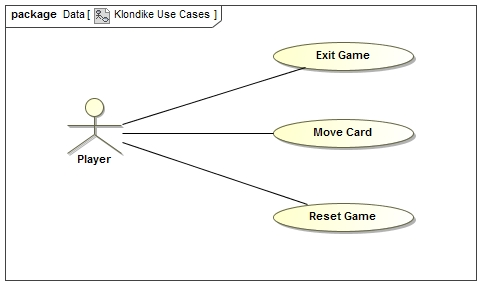
\includegraphics[width=13cm]{DomainModel/KlondikeUseCases.jpg}
   \caption{Acciones del Jugador}
   \label{fig:actions}
 \end{center}
 \end{figure}
\end{center}

No se ha considerado la acción ``Start Game'', ya que se asume que dicha acción existirá siempre, independientemente del dominio.

Por otro lado, el caso de uso ``Reset Game'' hace referencia al reparto de las cartas, tanto si es el reparto inicial como si es un reparto que el jugador realiza en mitad de la partida, puesto que quiere comenzar la partida de nuevo. Por tanto, se estima que, a nivel de modelo del dominio, los casos de uso principales son los mencionados anteriormente.

Las acciones en las que se reparten las cartas y se termina la partida no merecen mención especial, ya que son casos muy claros una vez conocido el funcionamiento del juego. Sin embargo, el modelo del dominio debe hacer hincapié en qué pasa cuando se posiciona una carta desde un mazo a otro dentro del juego.

En primer lugar, cabe indicar que hay una jerarquía de movimientos disponible dentro de este juego de cartas. De esta forma, se identifica el siguiente diagrama, que permite establecer, dentro del caso de uso ``Move Card'', los distintos tipos de movimientos posibles. Pueden observarse en la siguiente figura:

\begin{center}
 \begin{figure}[H]
 \begin{center}
   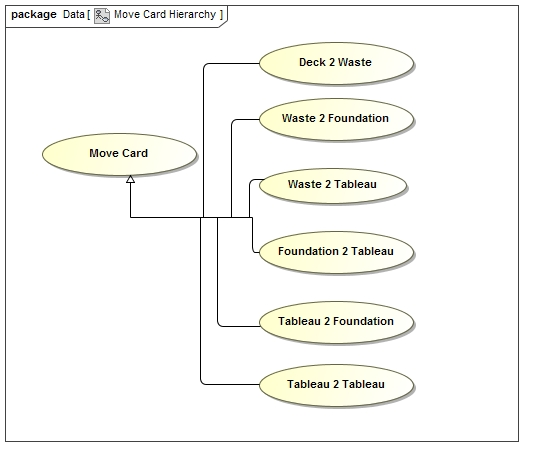
\includegraphics[width=14cm]{DomainModel/MoveCardHierarchy.jpg}
   \caption{Movimientos}
   \label{fig:movements}
 \end{center}
 \end{figure}
\end{center}

Una vez identificados los posibles movimientos, la realización de cada uno de los movimientos puede definirse como subacciones de ``Move Card''.

Una forma de especificar qué ocurre dentro de cada uno de los distintos movimientos es a través de diagramas de estados. A continuación, se muestran los estados que definen el problema del dominio para cada uno de los movimientos:

\begin{center}
 \begin{figure}[H]
 \begin{center}
   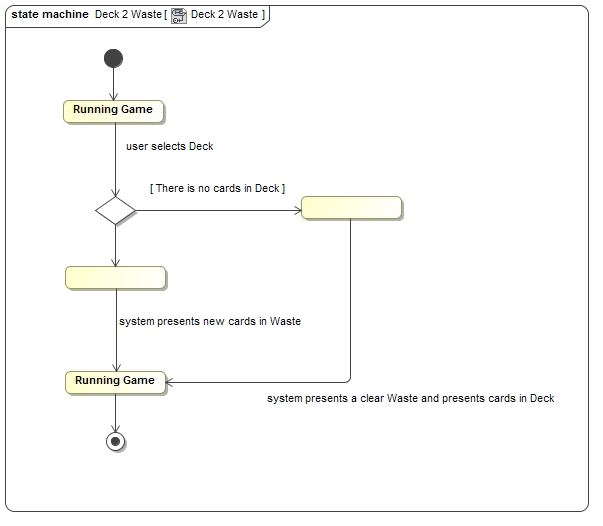
\includegraphics[width=14cm]{DomainModel/Deck2Waste.jpg}
   \caption{Deck To Waste}
   \label{fig:deck2waste}
 \end{center}
 \end{figure}
\end{center}
\begin{center}

\begin{figure}[H]
 \begin{center}
   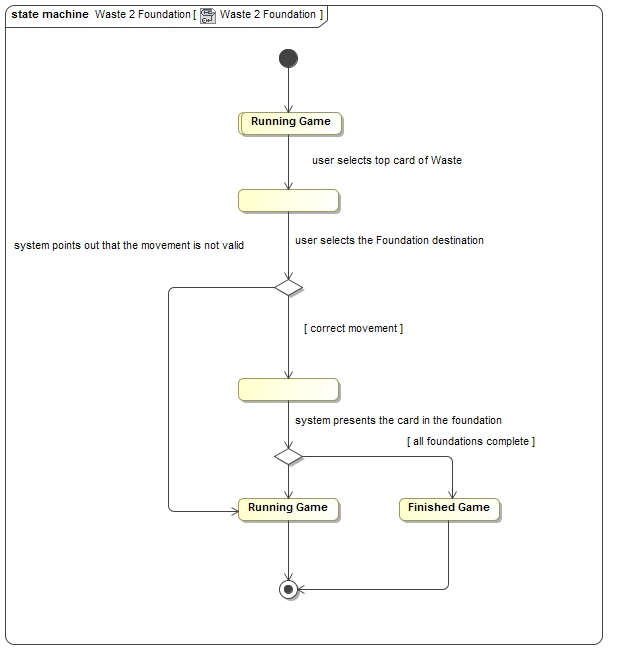
\includegraphics[width=14cm]{DomainModel/Waste2Foundation.jpg}
   \caption{Waste To Foundation}
   \label{fig:waste2foundation}
 \end{center}
 \end{figure}
\end{center}

\begin{center}
 \begin{figure}[H]
 \begin{center}
   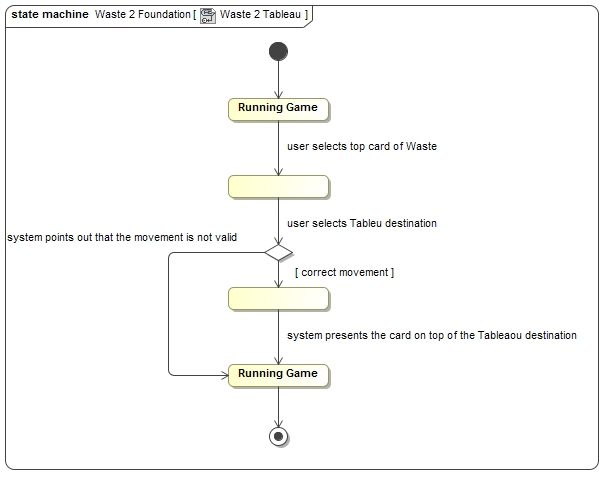
\includegraphics[width=14cm]{DomainModel/Waste2Tableau.jpg}
   \caption{Waste To Tableau}
   \label{fig:waste2tableau}
 \end{center}
 \end{figure}
\end{center}

\begin{center}
 \begin{figure}[H]
 \begin{center}
   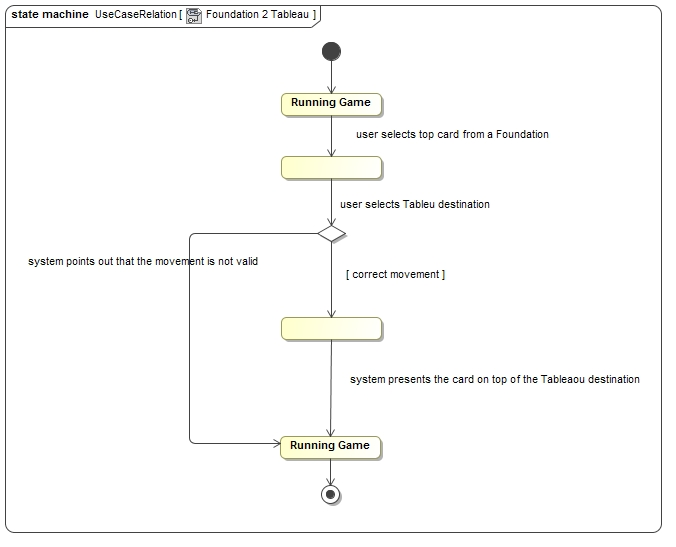
\includegraphics[width=14cm]{DomainModel/Foundation2Tableau.jpg}
   \caption{Foundation To Tableau}
   \label{fig:foundation2tableau}
 \end{center}
 \end{figure}
\end{center}

\begin{center}
 \begin{figure}[H]
 \begin{center}
   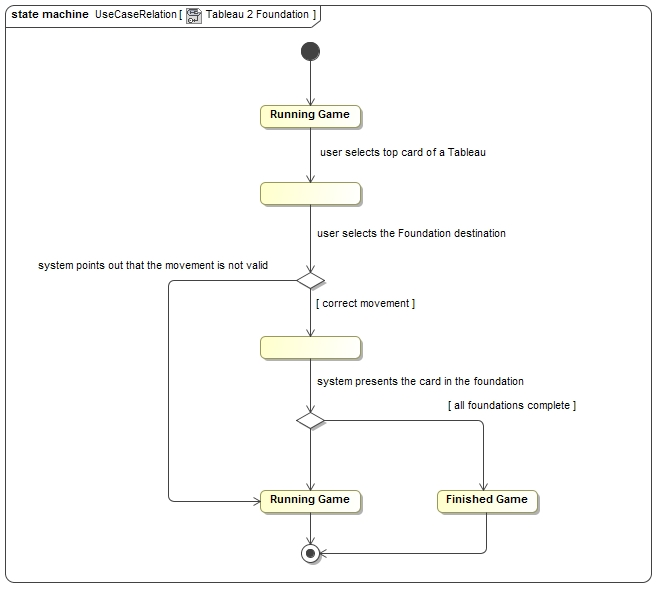
\includegraphics[width=14cm]{DomainModel/Tableau2Foundation.jpg}
   \caption{Tableau To Foundation}
   \label{fig:tableau2foundation}
 \end{center}
 \end{figure}
\end{center}

\begin{center}
 \begin{figure}[H]
 \begin{center}
   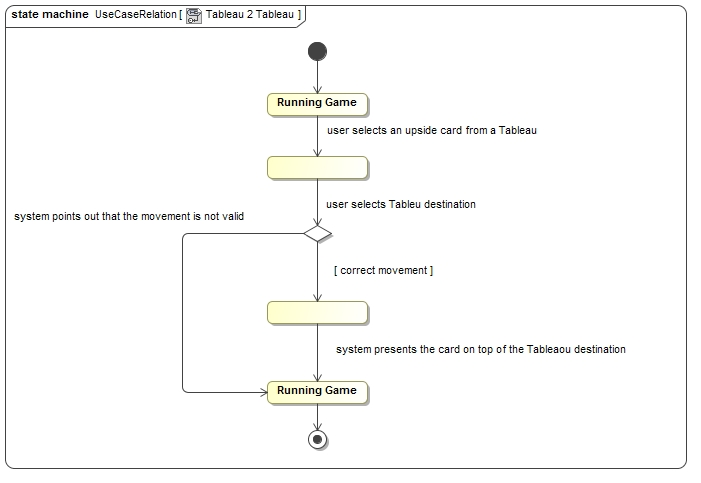
\includegraphics[width=14cm]{DomainModel/Tableau2Tableau.jpg}
   \caption{Tableau To Tableau}
   \label{fig:tableau2tableau}
 \end{center}
 \end{figure}
\end{center}

\pagebreak

\section{Modelo de Casos de Uso}

\pagebreak

\section{Modelo de Análisis}



Desde el punto de vista del modelo de análisis, existen dos tipos de diagramas principales que permiten realizar 
\end{document}
